%
% $Id: outro.tex 2771 2008-10-15 16:29:47Z sliske $
%
\addtocontents{toc}{\protect\newpage}
% start the appendix (changes section numbering, and others)
\appendix
% use different page style
\pagestyle{appendixstyle}
%reset acronym counter
% \acresetall % really? (by stefan)

%list of figures
%

\listoffigures
%\cleardoublepage

%
% list of tables
%

\listoftables
%\cleardoublepage

%
% list of algorithms
%

\listofalgorithms
%\cleardoublepage

%
% list of abbreviations
%

\iflanguage{ngerman}
{
\chapter{Abkürzungsverzeichnis}
}{
\chapter{Abbreviations}
}
\begin{acronym}[skbufflonglon]
\acro{API}{Application Programming Interface}
\acro{AMQP}{Advanced Message Queue Protocol}
\acro{ARM}{Advanced \acs{RISC} Machines}
\acro{BCC}{BPF Compiler Collection}
\acro{BIND}{Berkeley Internet Name Domain Server}
 \acro{BPF}{Berkeley Packet Filter}
 \acro{BPF CORE}{BPF Compile Once Run Everywhere}
 \acro{BTF}{BPF Type Format}
 \acro{cBPF}{classical Berkeley Packet Filter}
 \acro{CPU}{Central Processing Unit}
 \acro{DNS}{Domain Name System}
 \acro{DUT}{Device under Test}
 \acro{DDIO}{Direct Data Input Output}
 \acro{DoS}{Denial of Service}
 \acro{DDoS}{Distributed Denial of Service}
 \acro{DMA}{Direct Memory Access}
 \acro{DPDK}{Data Plane Development Kit}
 \acro{eBPF}{extended Berkeley Packet Filter}
 \acro{ESP}{Encapsulating Security Payload}
 \acro{FIFO}{First in First out}
 \acro{HIDS}{Host-based Intrusion Detection System}
 \acro{HTTP}{Hypertext Transfer Protocol}
 \acro{IANA}{Internet Assigned Numbers Authority}
 \acro{IDS}{Intrusion Detection System}
 \acro{IEEE}{Institute of Electrical and Electronics Engineers}
 \acro{IP}{Internet Protocol}
 \acro{IPC}{Inter-Process Communication}
 \acro{IPS}{Intrusion Prevention System}
 \acro{IPsec}{\acs{IP} Security}
 \acro{IPv4}{Internet Protocol Version 4}
 \acro{IPv6}{Internet Protocol Version 6}
 \acro{IO}{Input / Output}
 \acro{ISP}{Internet Service Provider}
 \acro{JIT}{Just in Time}
 \acro{LLVM}{Low Level Virtual Machine}
 \acro{MAC}{Media Control Access}
 \acro{MPPS}{Million Packets Per Second}
 \acro{MTU}{Maximum Transfer Unit}
 \acro{NAPI}{New \acs{API}}
 \acro{API}{Application Programming Interface}
 \acro{NAT}{Network Address Translation}
 \acro{NIC}{Network Interface Card}
 \acro{NIDS}{Network-based Intrusion Detection System}
 \acro{NSD}{Name Server Daemon}
 \acro{pcap}{Packet Capture}
 \acro{OS}{Operating System}
 \acro{OSI}{Open Systems Interconnection}
 \acro{PCI}{Peripheral Component Interconnect}
 \acro{PoC}{Proof of Concept}
 \acro{PPS}{Packets per Second}
 \acro{RAM}{Random Access Memory}
 \acro{regex}{regular expression}
 \acro{RIPE}{Réseaux IP Européens (European \ac{IP} Networks)}
 \acro{RISC}{Reduced Instruction Set Computer}
 \acro{RFC}{Request for Comments}
 \acro{Regex}{Regular Expression}
 \acro{skbuff}[\texttt{sk\textunderscore buff}]{Socket Buffer}
 \acro{SSH}{Secure Shell}
 \acro{SIEM}{Security Information and Event Management}
 \acro{tc}[\texttt{tc}]{Traffic Control}
 \acro{TCP}{Transmission Control Protocol}
 \acro{TLS}{Transport Layer Security}
 \acro{UDP}{User Datagram Protocol}
 \acro{VM}{Virtual Machine}
 \acro{VLAN}{Virtual Local Area Network}
 \acro{XDP}{eXpress Data Path}
 \acro{RAM}{Random Access Memory}

 \acrodefplural{OS}[OS's]{Operating Systems}
 \acrodefplural{IPS}[IPS]{Intrusion Detection Systems}
 \acrodefplural{HIDS}[HIDS]{Host-based Intrusion Detection Systems}
 \acrodefplural{NIDS}[NIDS]{Network-based Intrusion Detection Systems}
 \acrodefplural{API}[APIs]{Application Programming Interfaces}


\end{acronym}
%\begingroup
%\let\clearpage\relax
\chapter{Source Files}
For the sake of not having to chop down a forest to print this thesis, no full source files will be appended.
The source code is available in a git repository at: \href{https://gitup.uni-potsdam.de/raatschen/bachelorarbeit}{https://gitup.uni-potsdam.de/raatschen/bachelorarbeit}.
Access can be requested through me, or the second supervisor Max Schrötter.
%\endgroup

\chapter{Measurements}


\begin{figure}[h!p]
	
	\centering
	\scriptsize
	\begin{tabular}{c}
    	\centerline{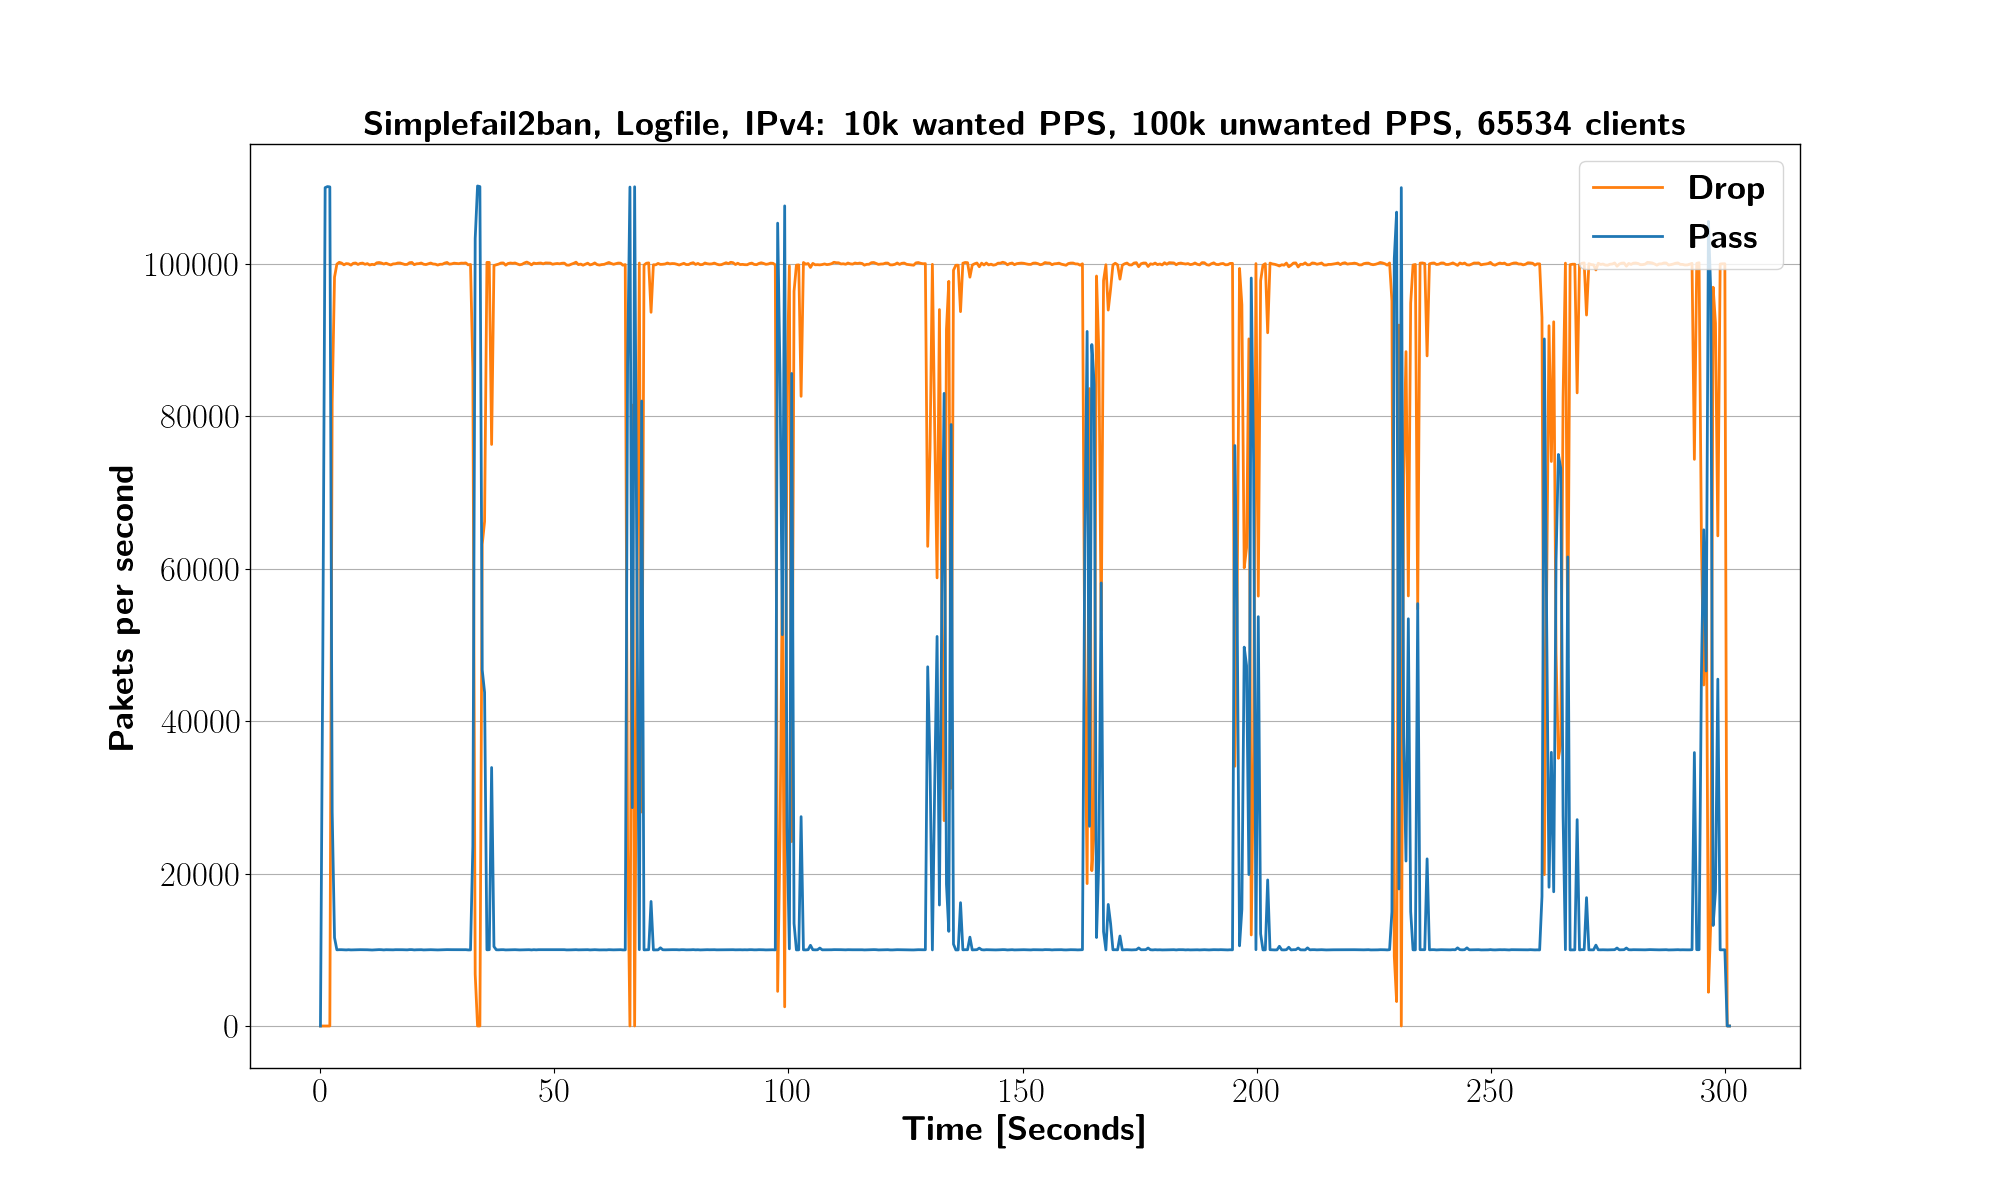
\includegraphics[width=1.2\textwidth]{images/simplefail2ban_disk_ipv4_v10k_iv100k_c65534.png}}
	\end{tabular}
	\begin{tabular}{lllll}
		\toprule
		\textbf{Total packets [$10^6$]} & \textbf{Packets dropped [$10^6$]} & \textbf{Relative drop [\%]} & \textbf{Log messages [$10^6$]} & \textbf{CPU [seconds]} \\ \midrule 
		33 & 27.93 & 99.59 & 2.07 & 10.51 \\
		\bottomrule
	\end{tabular}
	\caption[Simplefail2ban, Logfile IPv4, 100k \ac{PPS}]{Simplefail2ban Logfile \ac{IPv4}, 10 thousand unwanted \ac{PPS}, 100 thousand wanted \ac{PPS}, 65534 clients.}
	\label{fig:simplefail2ban:disk:ip4:100k}
\end{figure}

\begin{figure}[h!]
	\centering
	\scriptsize
	\begin{tabular}{c}
    	\centerline{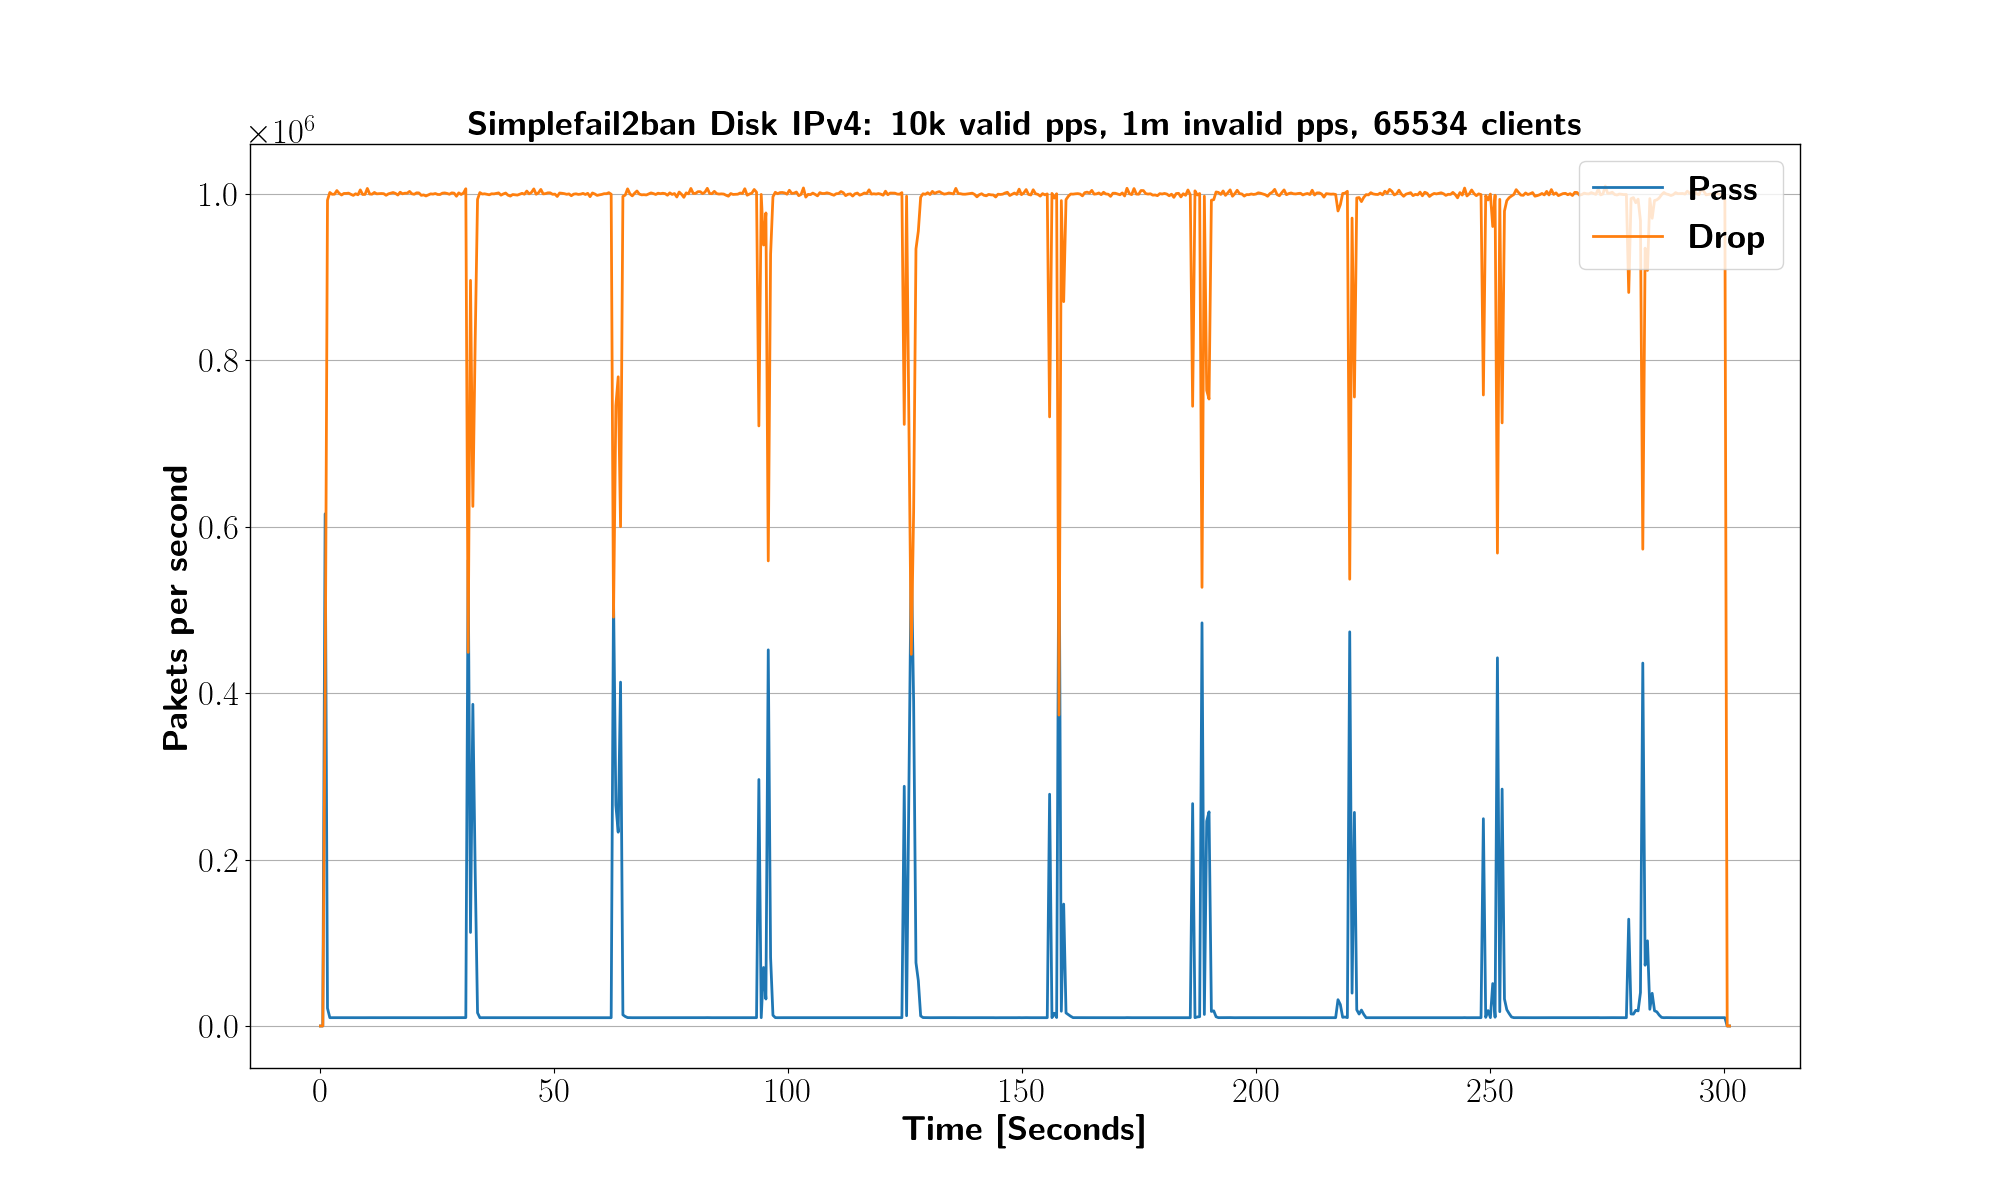
\includegraphics[width=1.2\textwidth]{images/simplefail2ban_disk_ipv4_v10k_iv1m_c65534.png}}
    \end{tabular}
	\begin{tabular}{lllll}
		\toprule
		\textbf{Total packets [$10^6$]} & \textbf{Packets dropped [$10^6$]} & \textbf{Relative drop [\%]} & \textbf{Log messages [$10^6$]} & \textbf{CPU [seconds]} \\ \midrule 
		303 & 294.43 & 98.79 & 4.7 & 14.99 \\
		\bottomrule
	\end{tabular}
	\caption[Simplefail2ban, Logfile IPv4, 1m \ac{PPS}]{Simplefail2ban Logfile \ac{IPv4}, 10 thousand unwanted \ac{PPS}, 1 million wanted \ac{PPS}, 65534 clients.}
	\label{fig:simplefail2ban:disk:ip4:1m}
\end{figure}

\begin{figure}[h!]
	\centering
	\scriptsize
	\begin{tabular}{c}
    	\centerline{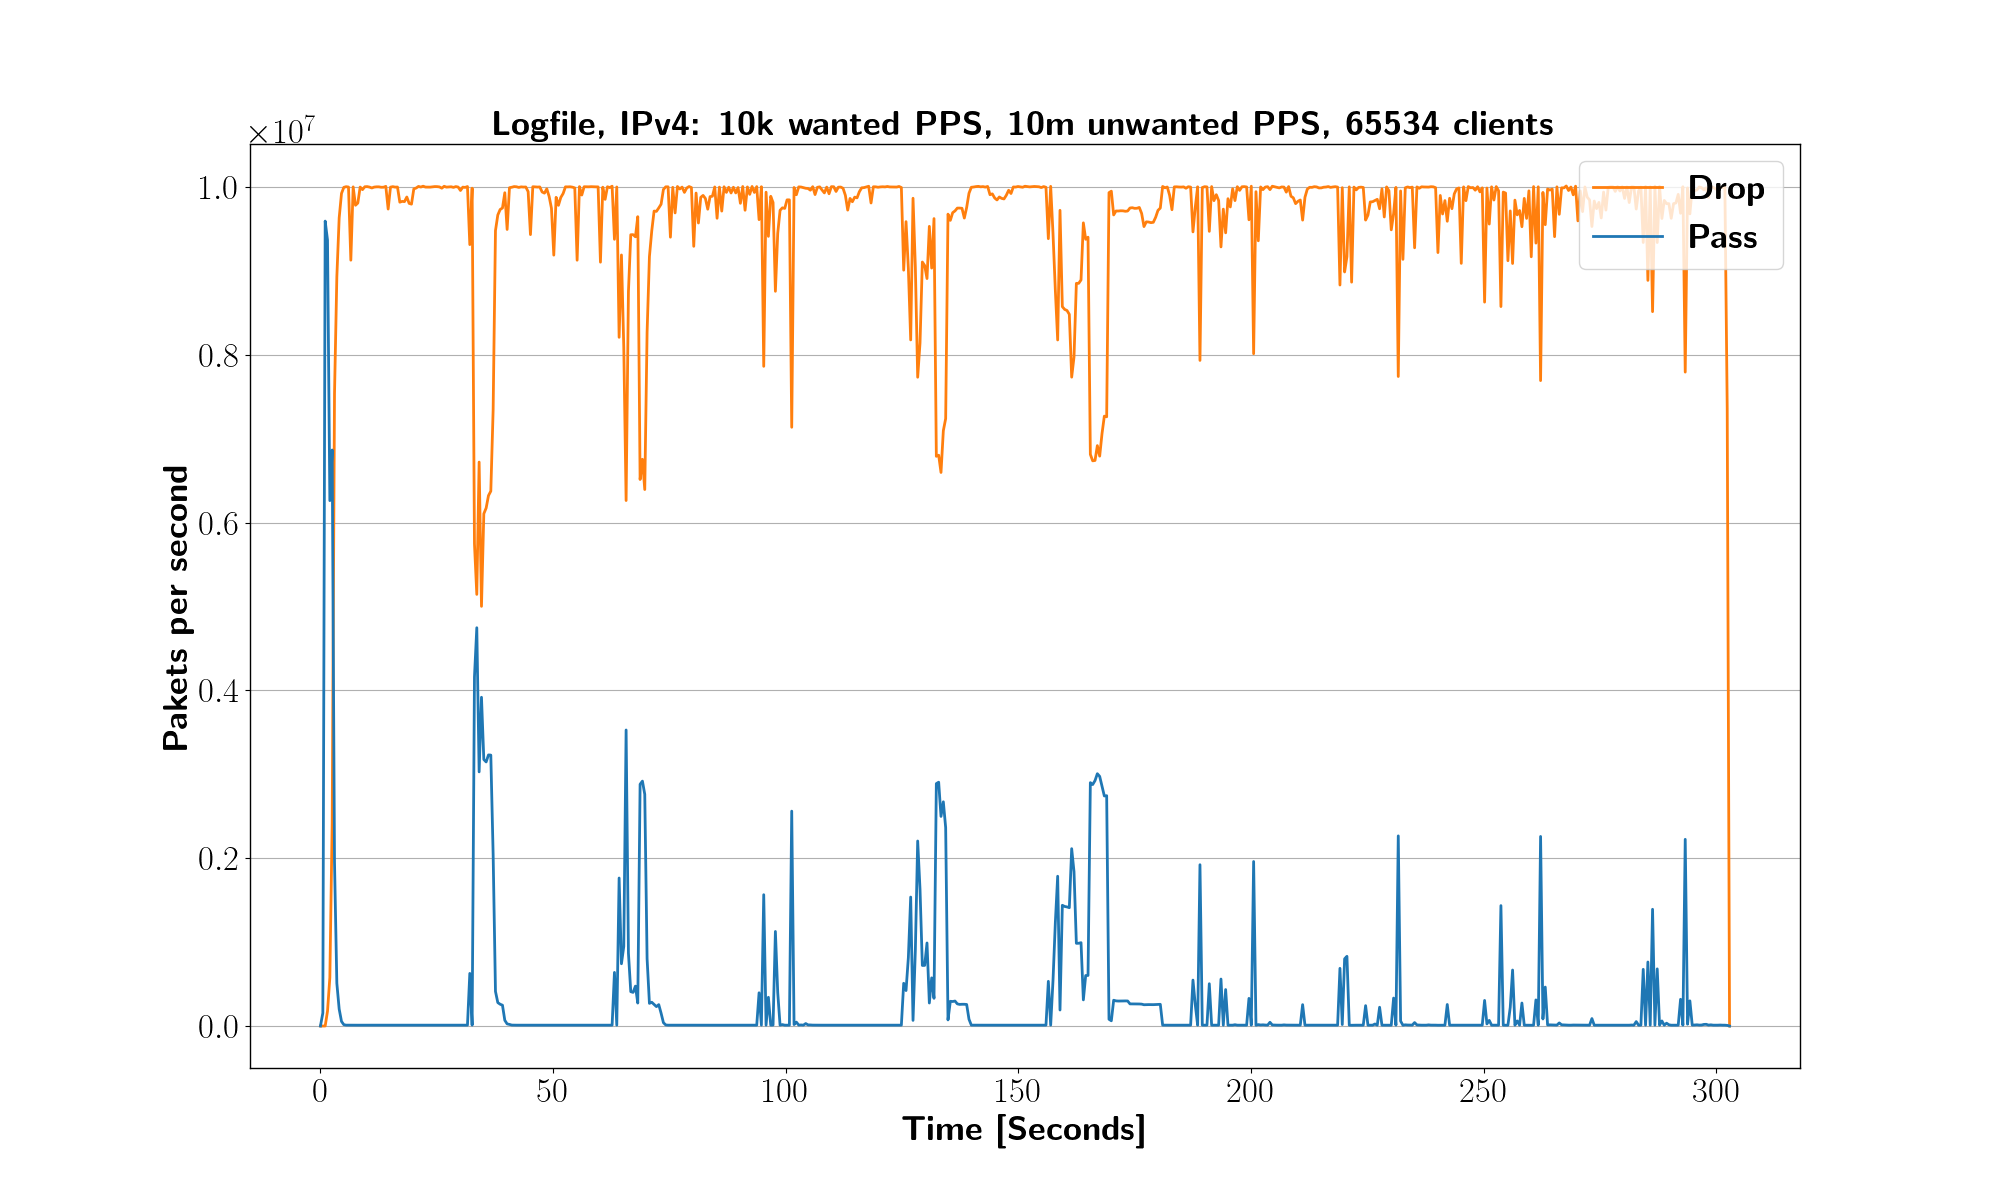
\includegraphics[width=1.2\textwidth]{images/simplefail2ban_disk_ipv4_v10k_iv10m_c65534.png}}
	\end{tabular}
	\begin{tabular}{lllll}
		\toprule
		\textbf{Total packets [$10^6$]} & \textbf{Packets dropped [$10^6$]} & \textbf{Relative drop [\%]} & \textbf{Log messages [$10^6$]} & \textbf{CPU [seconds]} \\ \midrule 
		2986.89 & 2884.14 & 96.72 & 34.39 & 83.72 \\
		\bottomrule
	\end{tabular}
	\caption[Simplefail2ban, Logfile IPv4, 10m \ac{PPS}]{Simplefail2ban Logfile \ac{IPv4}, 10 thousand unwanted \ac{PPS}, 10 million wanted \ac{PPS}, 65534 clients.}
	\label{fig:simplefail2ban:disk:ip4:10m}
\end{figure}

\begin{figure}[!h]
	\centering
	\scriptsize
	\begin{tabular}{c}
    	\centerline{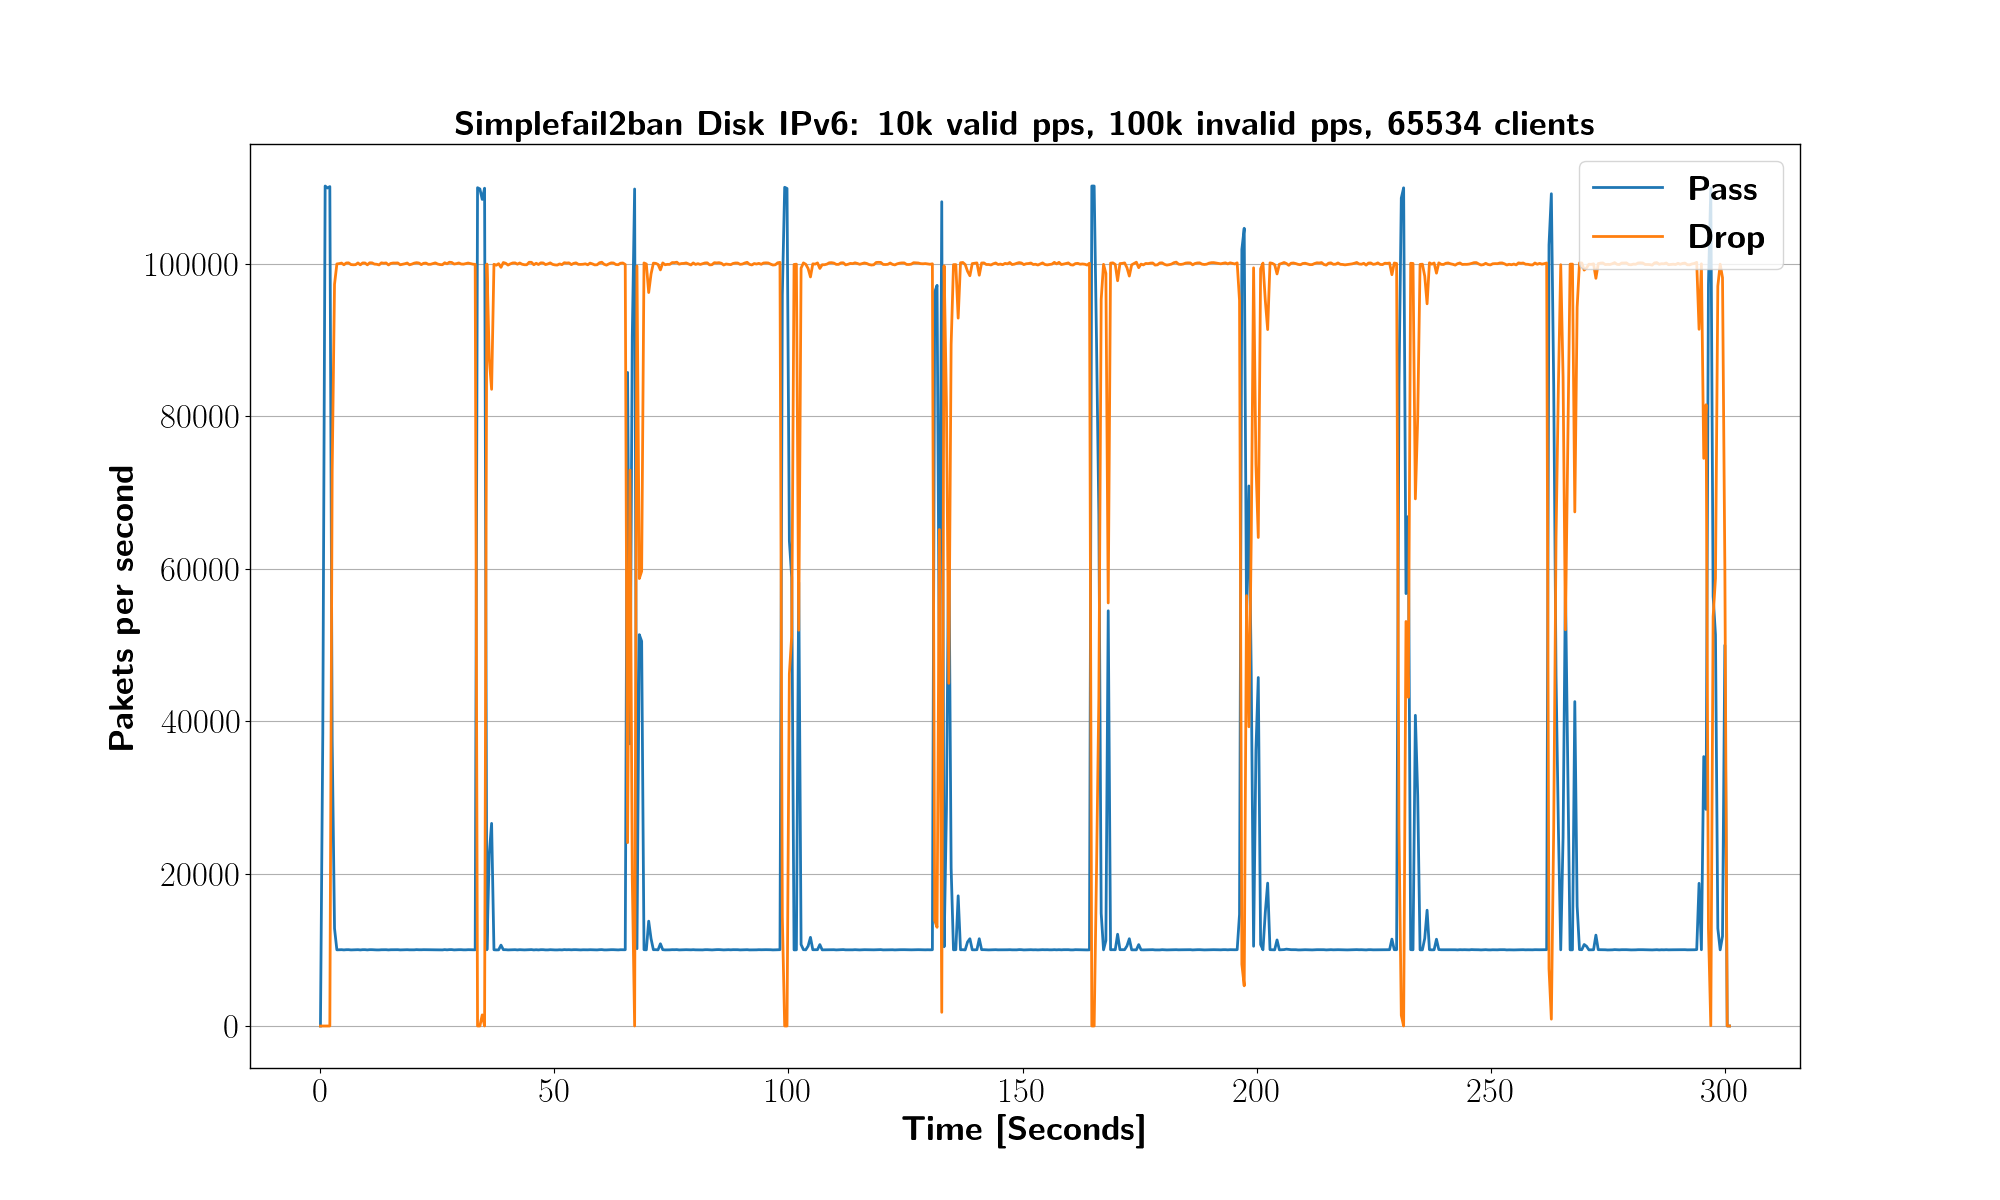
\includegraphics[width=1.2\textwidth]{images/simplefail2ban_disk_ipv6_v10k_iv100k_c65534.png}}
	\end{tabular}
	\begin{tabular}{lllll}
		\toprule
		\textbf{Total packets [$10^6$]} & \textbf{Packets dropped [$10^6$]} & \textbf{Relative drop [\%]} & \textbf{Log messages [$10^6$]} & \textbf{CPU [seconds]} \\ \midrule 
		33 & 27.96 & 99.67 & 2.04 & 11.75 \\
		\bottomrule
	\end{tabular}
	\caption[Simplefail2ban, Logfile IPv6, 100k \ac{PPS}]{Simplefail2ban Logfile \ac{IPv6}, 10 thousand wanted \ac{PPS}, 100 thousand unwanted \ac{PPS}, 65534 clients.}
	\label{fig:simplefail2ban:disk:ip6:100k}
\end{figure}

\begin{figure}[!h]
	\centering
	\scriptsize
	\begin{tabular}{c}
    	\centerline{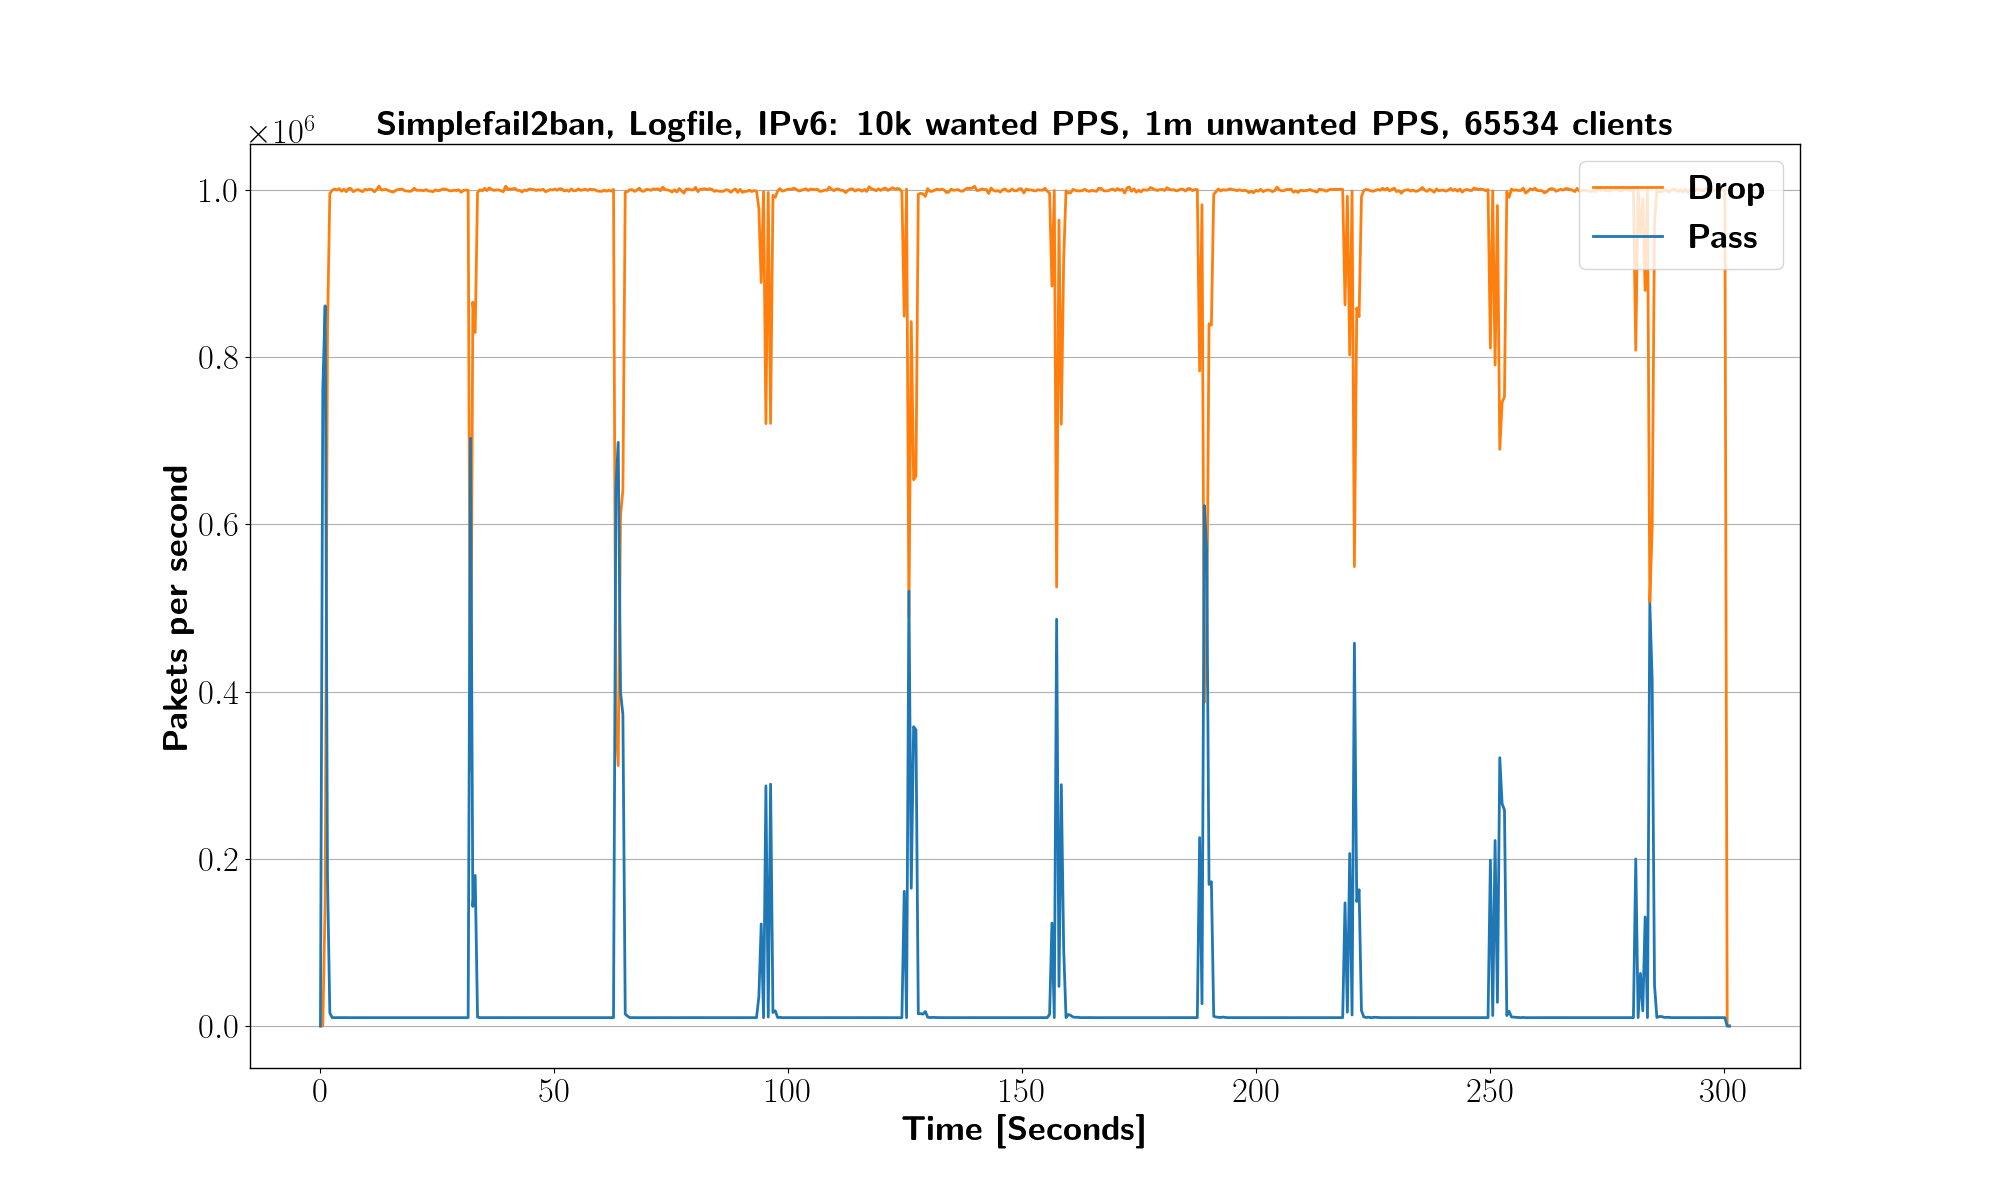
\includegraphics[width=1.2\textwidth]{images/simplefail2ban_disk_ipv6_v10k_iv1m_c65534.png}}
	\end{tabular}
	\begin{tabular}{lllll}
		\toprule
		\textbf{Total packets [$10^6$]} & \textbf{Packets dropped [$10^6$]} & \textbf{Relative drop [\%]} & \textbf{Log messages [$10^6$]} & \textbf{CPU [seconds]} \\ \midrule 
		303 & 293.49 & 98.48 & 5.58 & 21.08 \\
		\bottomrule
	\end{tabular}
	\caption[Simplefail2ban, Logfile IPv6, 1m \ac{PPS}]{Simplefail2ban Logfile \ac{IPv6}, 10 thousand wanted \ac{PPS}, 1 million unwanted \ac{PPS}, 65534 clients.}
	\label{fig:simplefail2ban:disk:ip6:1m}
\end{figure}

\begin{figure}[!h]
	\centering
	\scriptsize
	\begin{tabular}{c}
    	\centerline{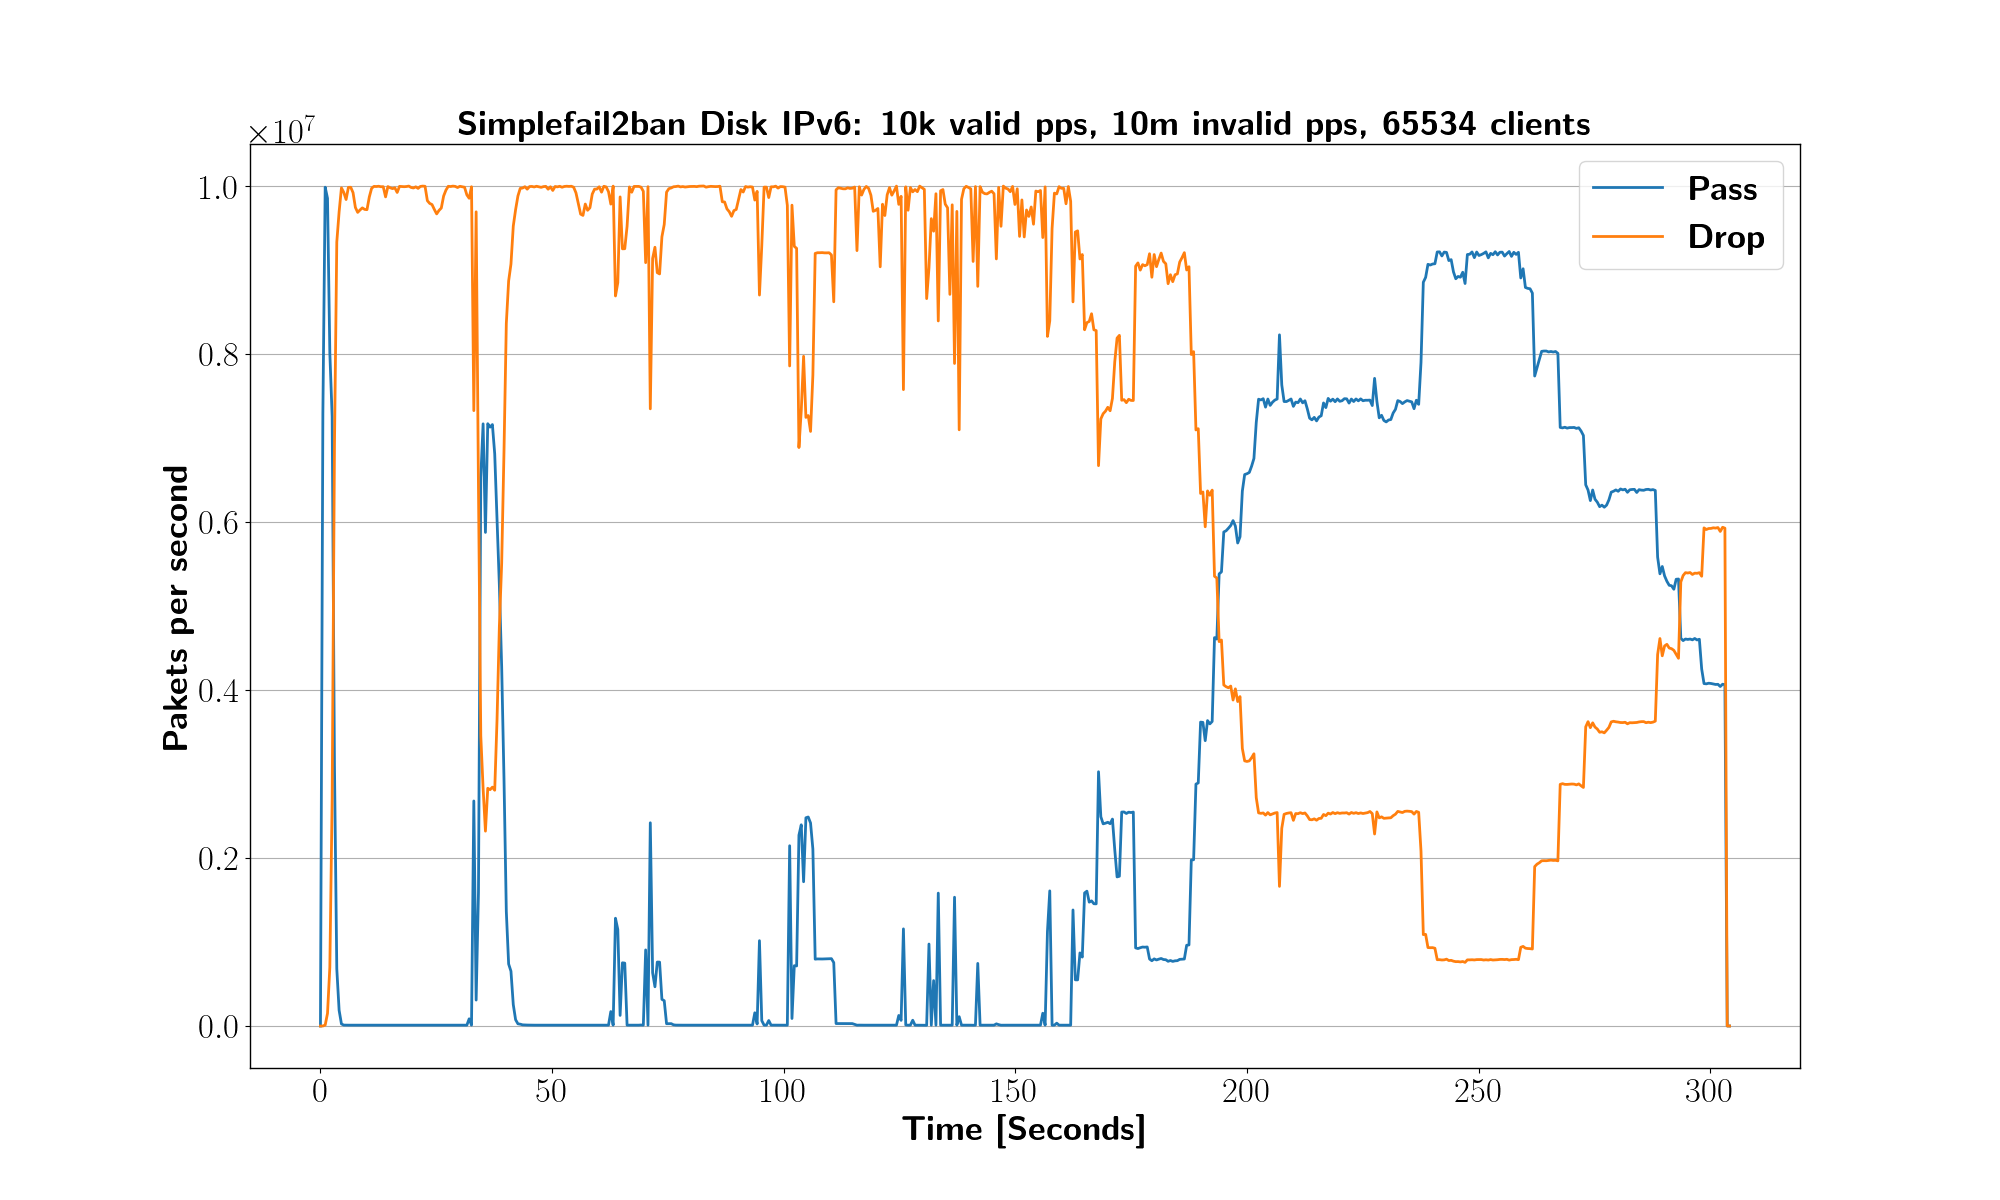
\includegraphics[width=1.2\textwidth]{images/simplefail2ban_disk_ipv6_v10k_iv10m_c65534.png}}
	\end{tabular}
	\begin{tabular}{lllll}
		\toprule
		\textbf{Total packets [$10^6$]} & \textbf{Packets dropped [$10^6$]} & \textbf{Relative drop [\%]} & \textbf{Log messages [$10^6$]} & \textbf{CPU [seconds]} \\ \midrule 
		2992.43 & 2065.28 & 69.13 & 205.4 & 346.73 \\
		\bottomrule
	\end{tabular}
	\caption[Simplefail2ban, Logfile IPv6, 10m \ac{PPS}]{Simplefail2ban Logfile \ac{IPv6}, 10 thousand wanted \ac{PPS}, 10 million unwanted \ac{PPS}, 65534 clients.}
	\label{fig:simplefail2ban:disk:ip6:10m}
\end{figure}


\begin{figure}[!h]
	\centering
	\scriptsize
	\begin{tabular}{c}
    	\centerline{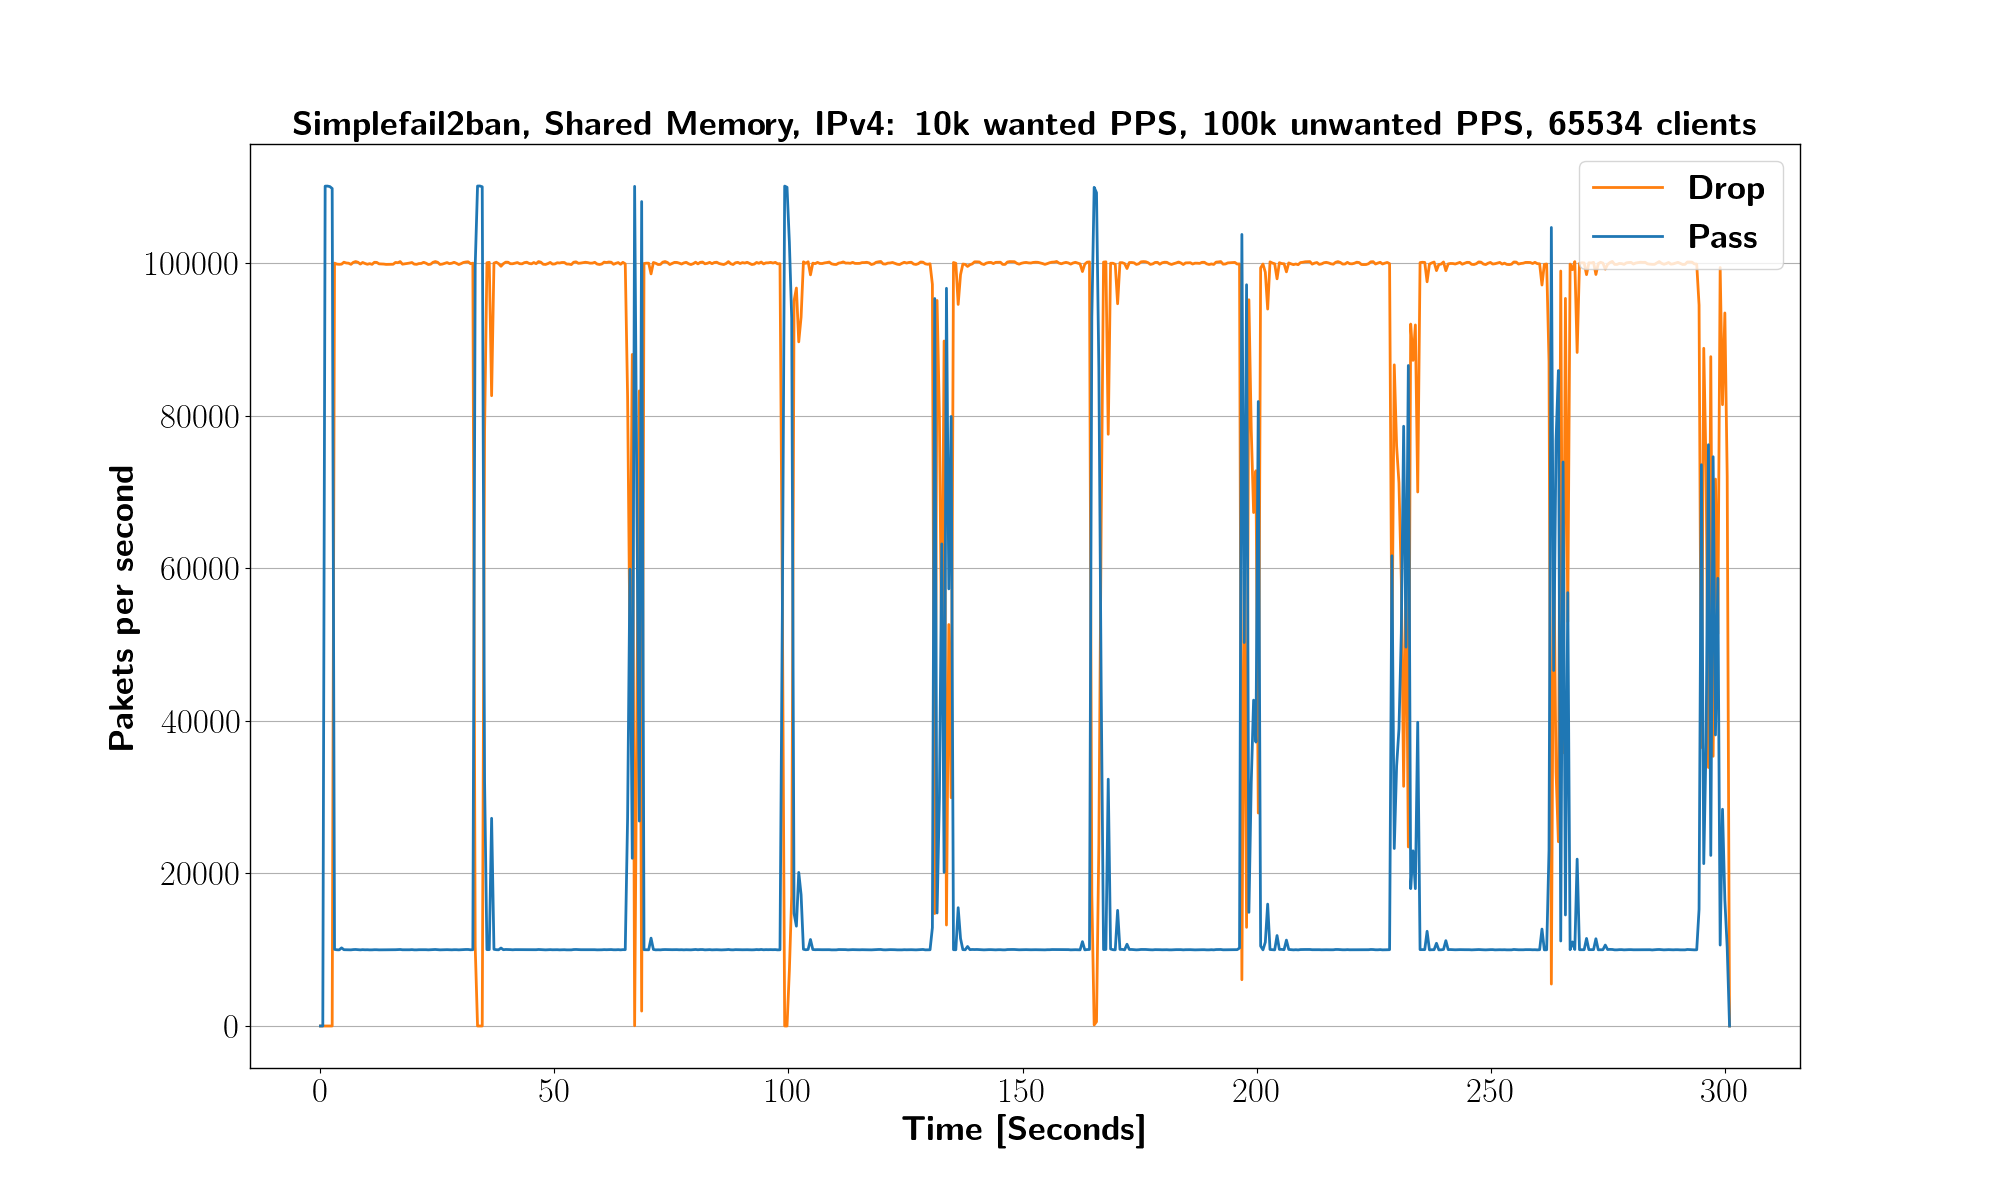
\includegraphics[width=1.2\textwidth]{images/simplefail2ban_shm_ipv4_v10k_iv100k_c65534.png}}
	\end{tabular}
	\begin{tabular}{lllll}
		\toprule
		\textbf{Total packets [$10^6$]} & \textbf{Packets dropped [$10^6$]} & \textbf{Relative drop [\%]} & \textbf{Log messages [$10^6$]} & \textbf{CPU [seconds]} \\ \midrule 
		33 & 27.95 & 99.64 & 2.05 & 13.68 \\
		\bottomrule
	\end{tabular}
	\caption[Simplefail2ban, Shared Memory, IPv4, 100k \ac{PPS}]{Simplefail2ban Shared Memory \ac{IPv4}, 10 thousand wanted \ac{PPS}, 100 thousand unwanted \ac{PPS}, 65534 clients.}
	\label{fig:simplefail2ban:shm:ip4:100k}
\end{figure}

\begin{figure}[!h]
	\centering
	\scriptsize
	\begin{tabular}{c}
    	\centerline{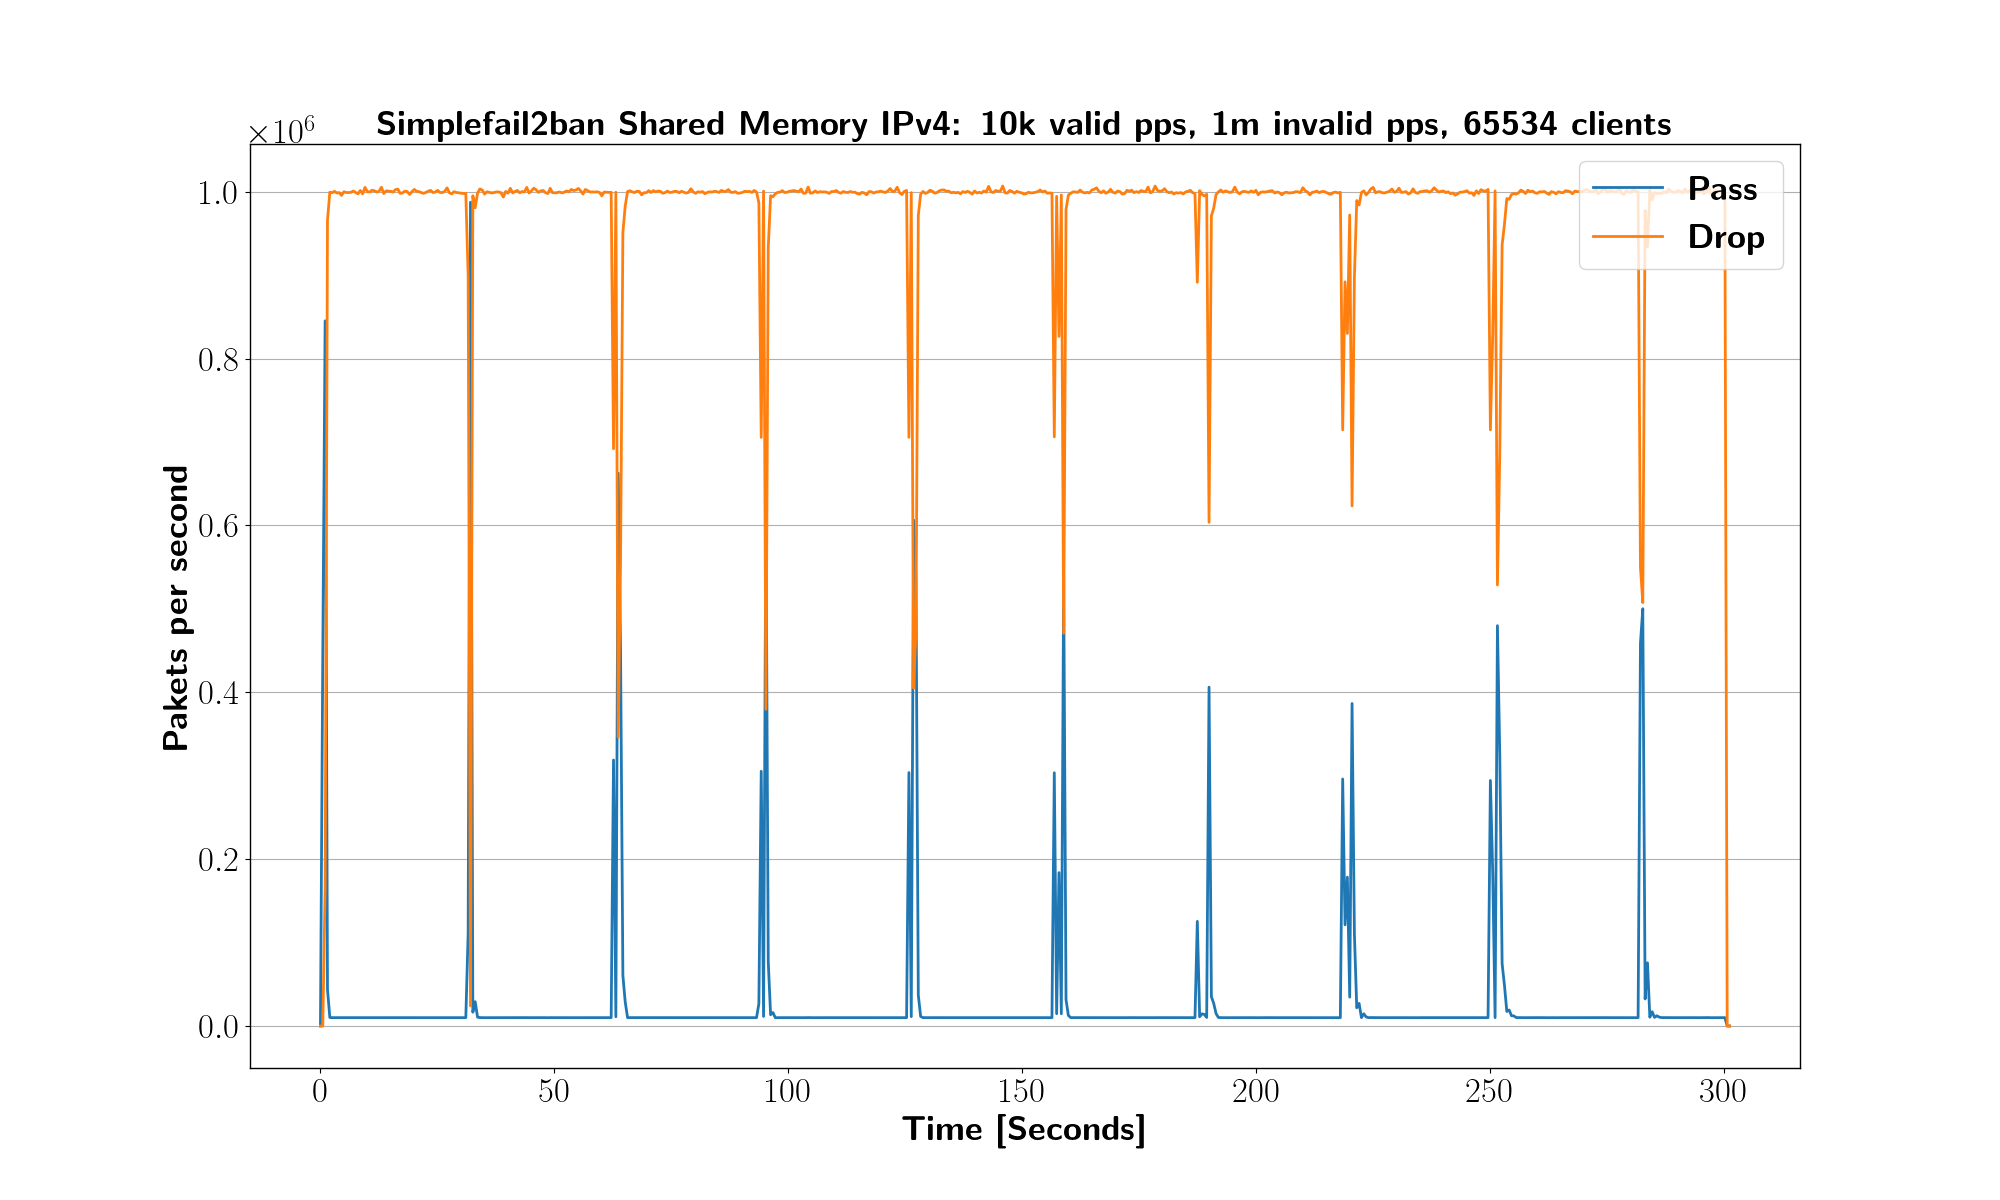
\includegraphics[width=1.2\textwidth]{images/simplefail2ban_shm_ipv4_v10k_iv1m_c65534.png}}
	\end{tabular}
	\begin{tabular}{lllll}
		\toprule
		\textbf{Total packets [$10^6$]} & \textbf{Packets dropped [$10^6$]} & \textbf{Relative drop [\%]} & \textbf{Log messages [$10^6$]} & \textbf{CPU [seconds]} \\ \midrule 
		303 & 294.34 & 98.88 & 4.61 & 15.52 \\
		\bottomrule
	\end{tabular}
	\caption[Simplefail2ban, Shared Memory, IPv4, 1m \ac{PPS}]{Simplefail2ban Shared Memory \ac{IPv4}, 10 thousand wanted \ac{PPS}, 10 million unwanted \ac{PPS}, 65534 clients.}
	\label{fig:simplefail2ban:shm:ip4:1m}
\end{figure}

\begin{figure}[!h]
	\centering
	\scriptsize
	\begin{tabular}{c}
    	\centerline{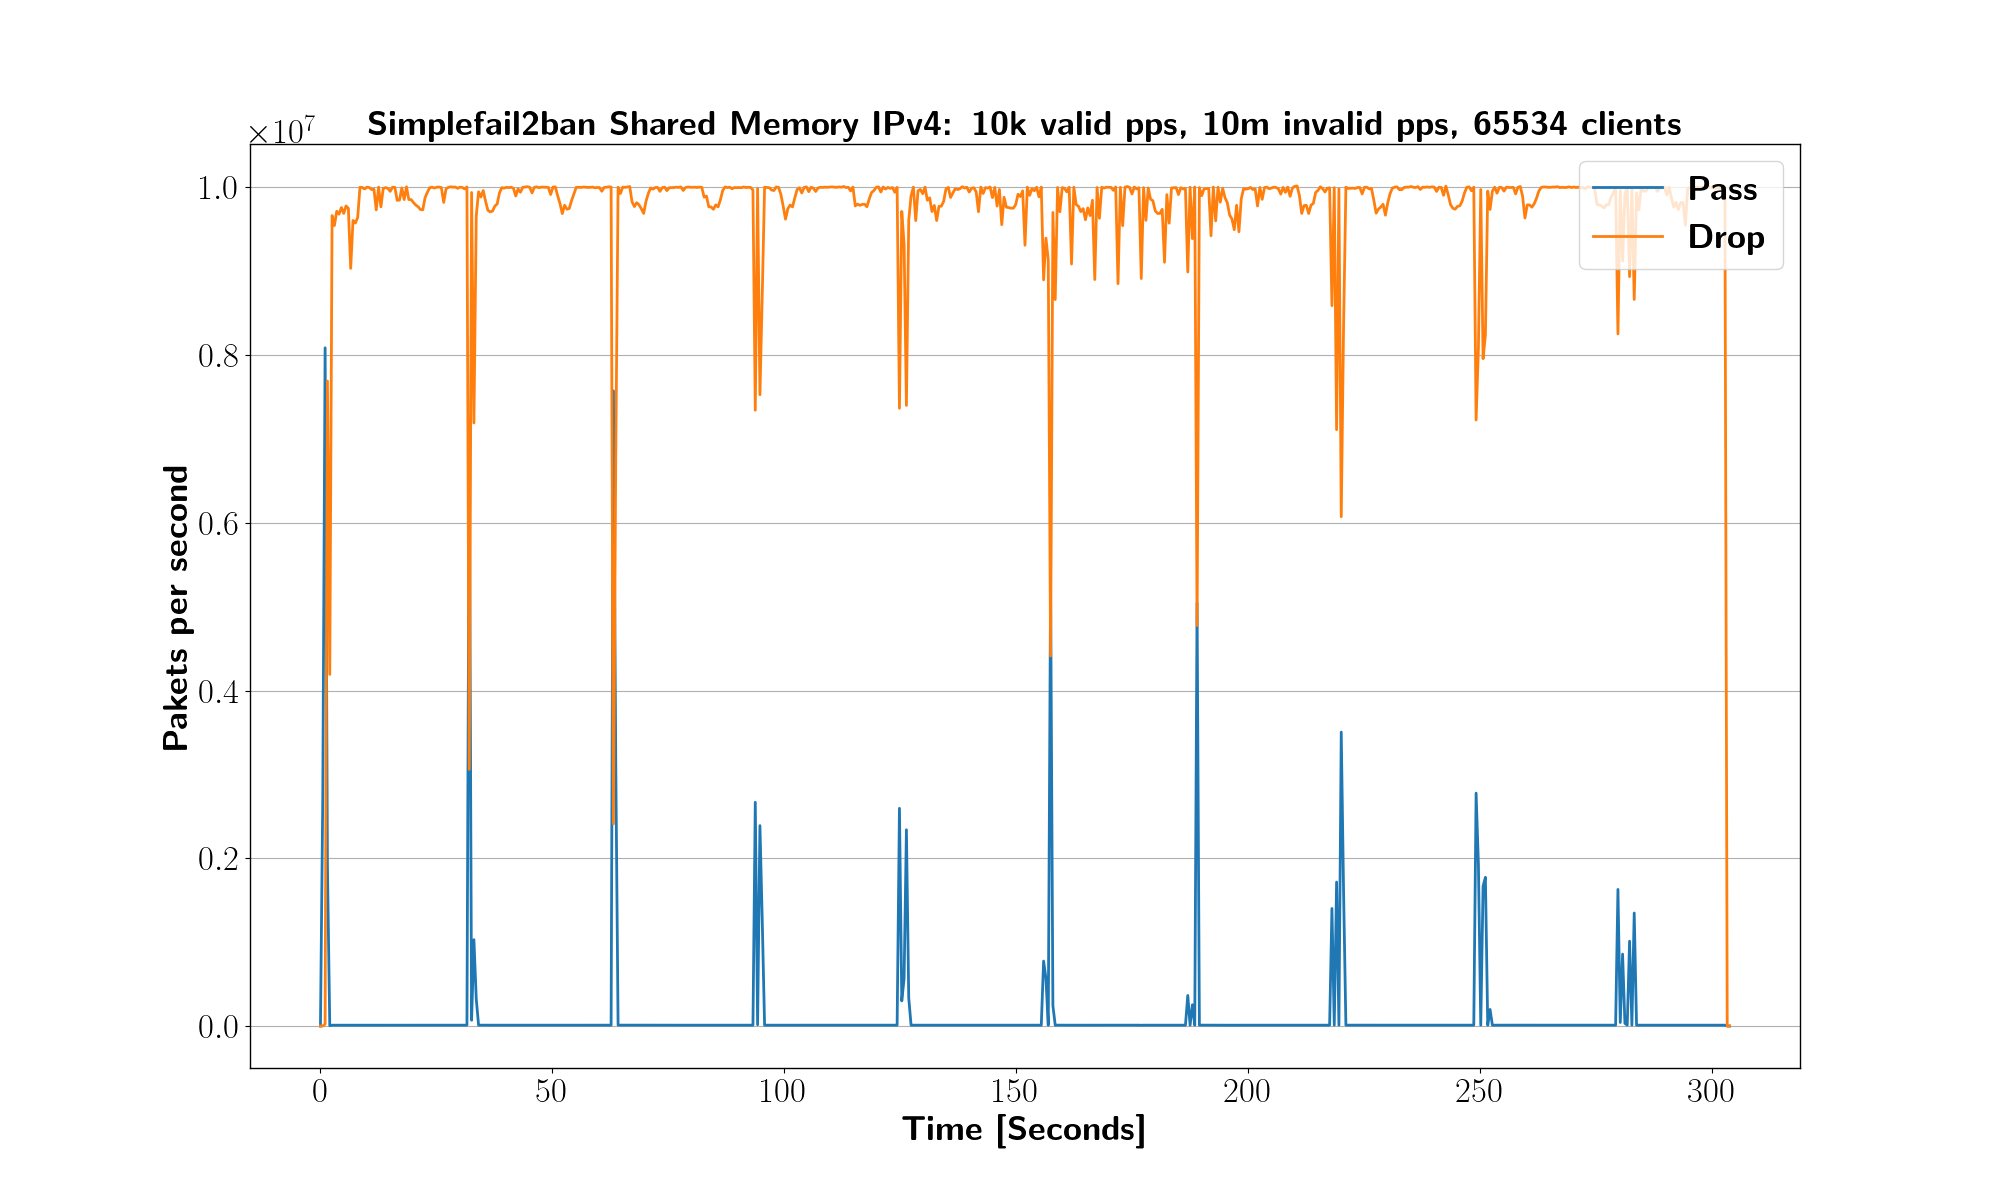
\includegraphics[width=1.2\textwidth]{images/simplefail2ban_shm_ipv4_v10k_iv10m_c65534.png}}
	\end{tabular}
	\begin{tabular}{lllll}
		\toprule
		\textbf{Total packets [$10^6$]} & \textbf{Packets dropped [$10^6$]} & \textbf{Relative drop [\%]} & \textbf{Log messages [$10^6$]} & \textbf{CPU [seconds]} \\ \midrule 
		2991.48 & 2948.51 & 96.72 & 7.69 & 25.59 \\
		\bottomrule
	\end{tabular}
	\caption[Simplefail2ban, Shared Memory, IPv4, 10m \ac{PPS}]{Simplefail2ban Shared Memory \ac{IPv4}, 10 thousand wanted \ac{PPS}, 10 million unwanted \ac{PPS}, 65534 clients.}
	\label{fig:simplefail2ban:shm:ip4:10m}
\end{figure}

\begin{figure}[!h]
	\centering
	\scriptsize
	\begin{tabular}{c}
    	\centerline{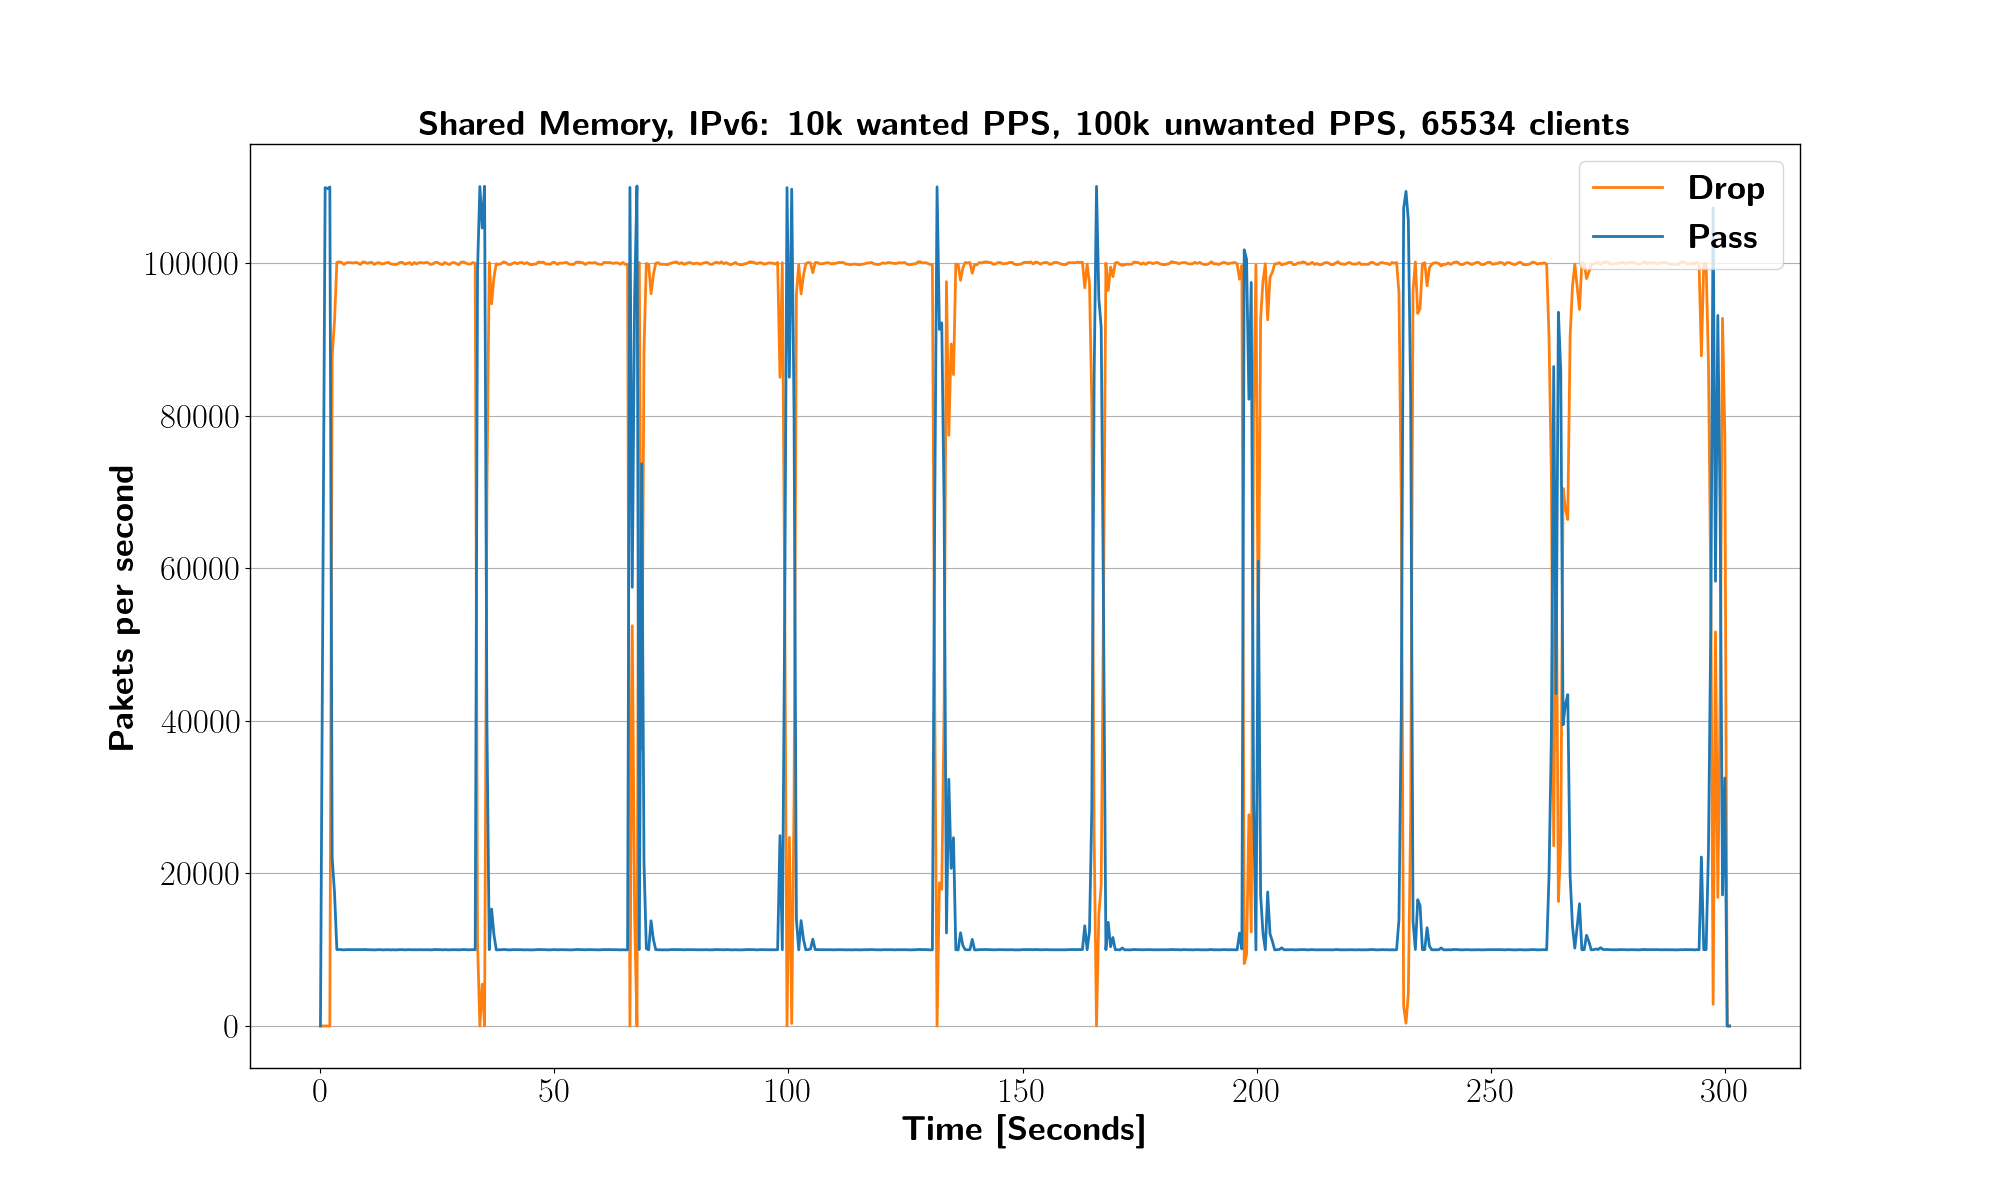
\includegraphics[width=1.2\textwidth]{images/simplefail2ban_shm_ipv6_v10k_iv100k_c65534.png}}
	\end{tabular}
	\begin{tabular}{lllll}
		\toprule
		\textbf{Total packets [$10^6$]} & \textbf{Packets dropped [$10^6$]} & \textbf{Relative drop [\%]} & \textbf{Log messages [$10^6$]} & \textbf{CPU [seconds]} \\ \midrule 
		33 & 27.95 & 99.67 & 2.05 & 15.55 \\
		\bottomrule
	\end{tabular}
	\caption[Simplefail2ban, Shared Memory, IPv6, 100k \ac{PPS}]{Simplefail2ban Shared Memory \ac{IPv6}, 10 thousand wanted \ac{PPS}, 100 thousand unwanted \ac{PPS}, 65534 clients.}
	\label{fig:simplefail2ban:shm:ip6:100k}
\end{figure}

\begin{figure}[!h]
	\centering
	\scriptsize
	\begin{tabular}{c}
    	\centerline{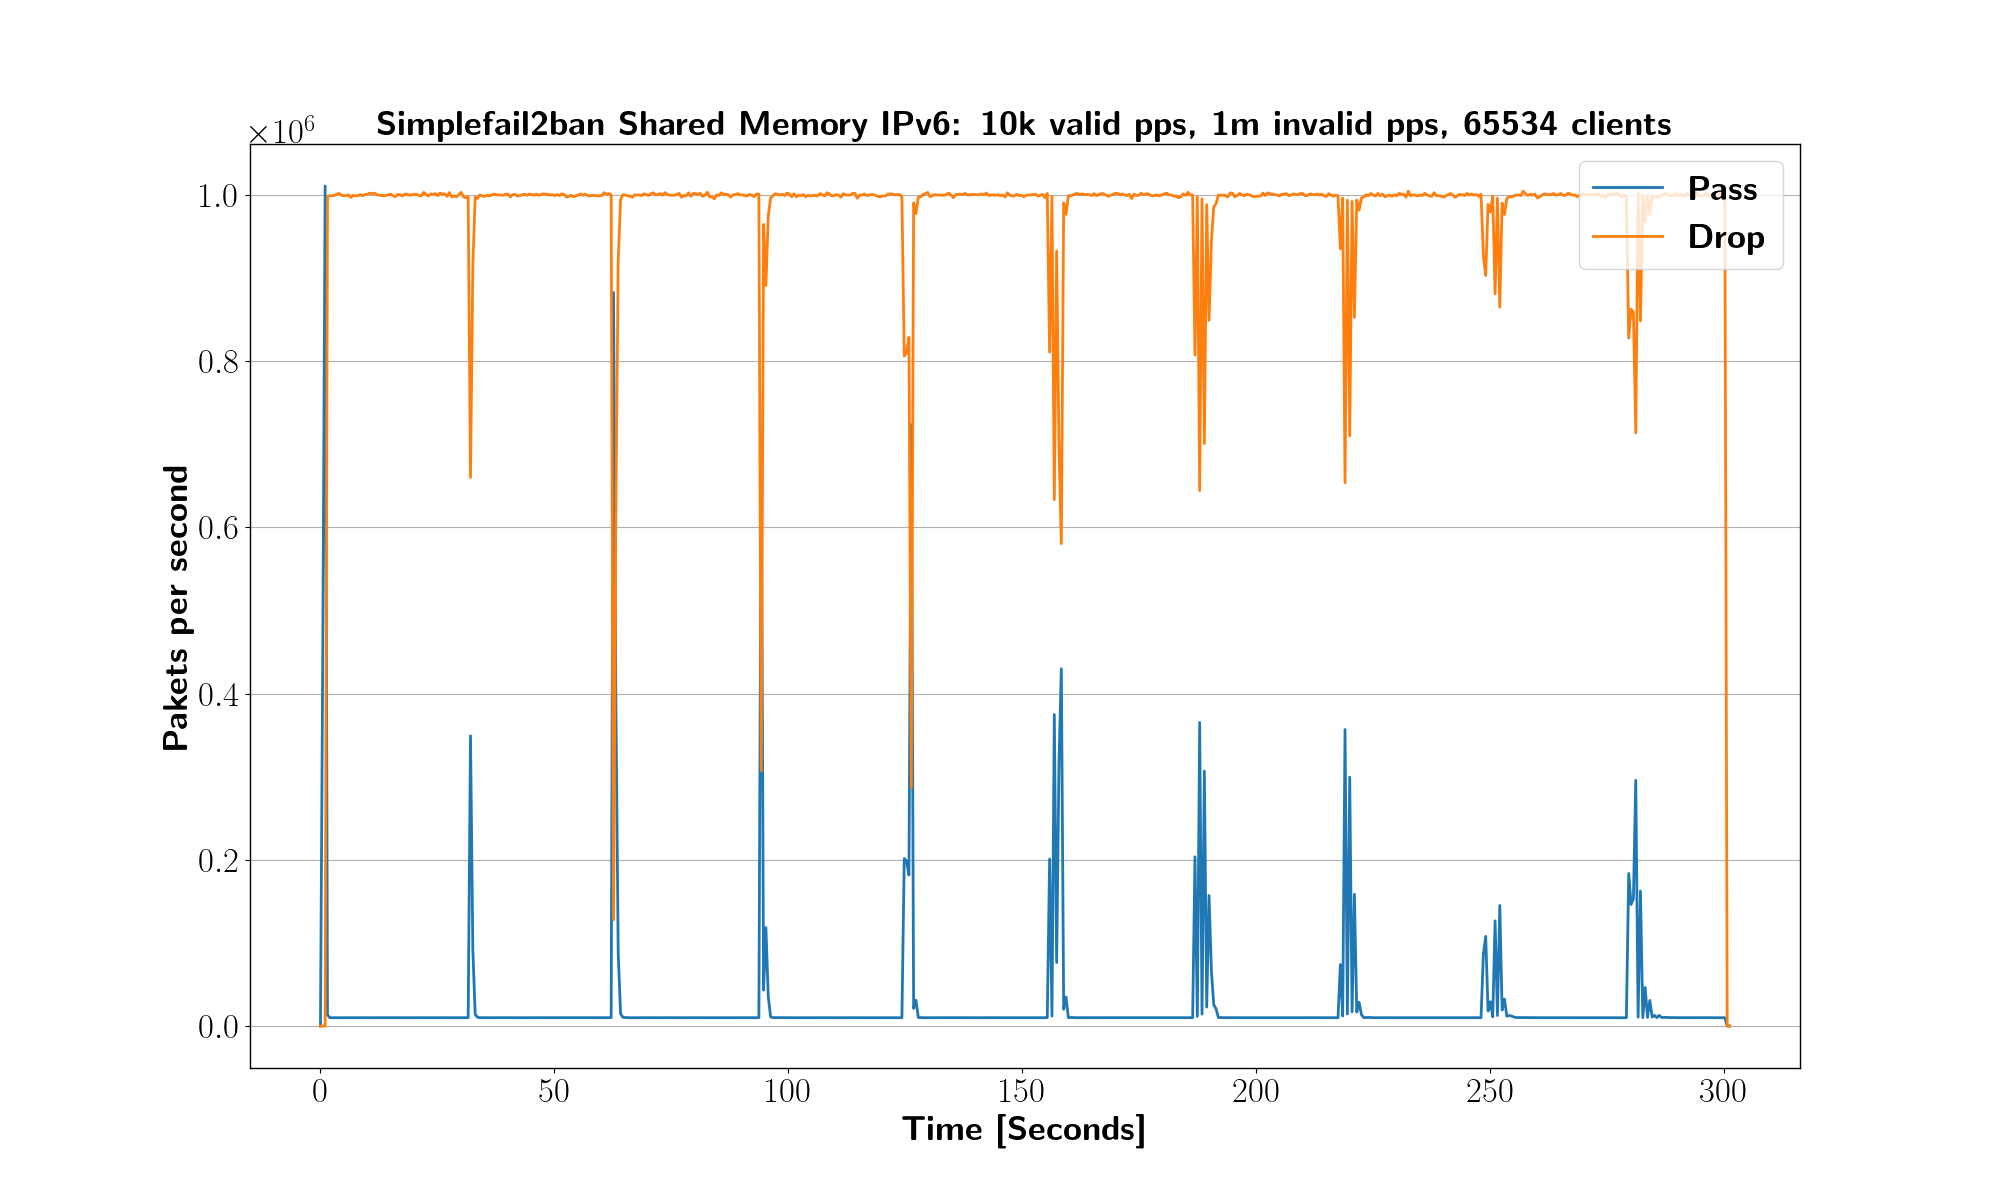
\includegraphics[width=1.2\textwidth]{images/simplefail2ban_shm_ipv6_v10k_iv1m_c65534.png}}
	\end{tabular}
	\begin{tabular}{lllll}
		\toprule
		\textbf{Total packets [$10^6$]} & \textbf{Packets dropped [$10^6$]} & \textbf{Relative drop [\%]} & \textbf{Log messages [$10^6$]} & \textbf{CPU [seconds]} \\ \midrule 
		303 & 294.77 & 98.9 & 4.39 & 17.46 \\
		\bottomrule
	\end{tabular}
	\caption[Simplefail2ban, Shared Memory, IPv6, 1m \ac{PPS}]{Simplefail2ban Shared Memory \ac{IPv6}, 10 thousand wanted \ac{PPS}, 1 million unwanted \ac{PPS}, 65534 clients.}
	\label{fig:simplefail2ban:shm:ip6:1m}
\end{figure}

\begin{figure}[!h]
	\centering
	\scriptsize
	\begin{tabular}{c}
    	\centerline{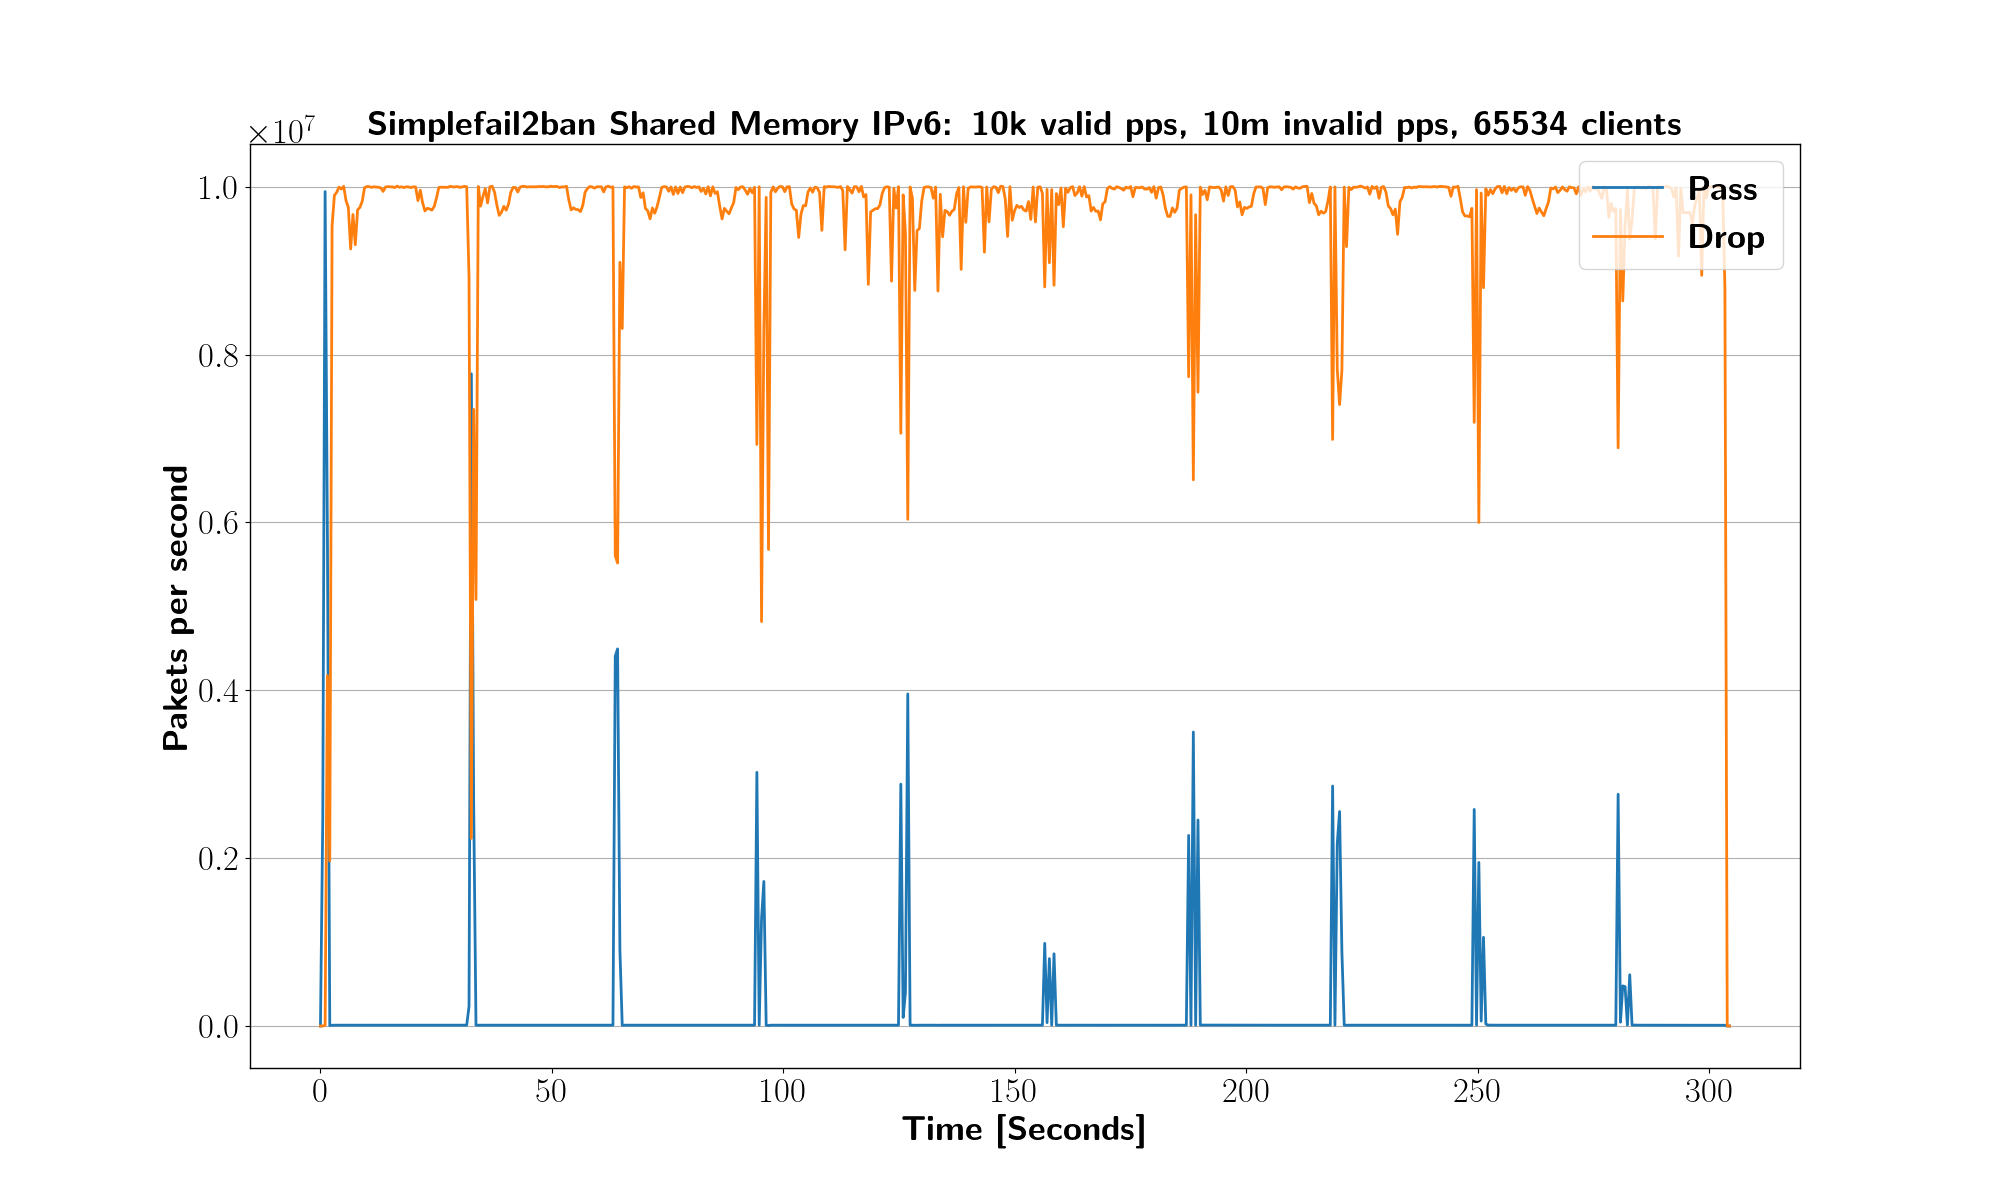
\includegraphics[width=1.2\textwidth]{images/simplefail2ban_shm_ipv6_v10k_iv10m_c65534.png}}
	\end{tabular}
	\begin{tabular}{lllll}
		\toprule
		\textbf{Total packets [$10^6$]} & \textbf{Packets dropped [$10^6$]} & \textbf{Relative drop [\%]} & \textbf{Log messages [$10^6$]} & \textbf{CPU [seconds]} \\ \midrule 
		2991.93 & 2947.1 & 98.66 & 8.88 & 32.36 \\
		\bottomrule
	\end{tabular}
	\caption[Simplefail2ban, Shared Memory, IPv6, 10m \ac{PPS}]{Simplefail2ban Shared Memory \ac{IPv6}, 10 thousand wanted \ac{PPS}, 10 million unwanted \ac{PPS}, 65534 clients.}
	\label{fig:simplefail2ban:shm:ip6:10m}
\end{figure}

%
% bibliography
%
\def\UrlBreaks{\do\/\do-}
% alphaurl is a special bibliography style which includes Hyperlinks 
% to papers
\begingroup
\sloppy
%\raggedright
\bibliographystyle{unsrt}
% bib file without extension
\bibliography{literature}
\endgroup


%\printindex 
